\section{Sphinx}
\todo{Iness: This entire subsection explains the original sphinx packet format, I think it's too much and can be reduced to 20\%. The rest can be either be deleted or used on how you construct the decentralized scheme}
Sphinx packets consist of a header and an encrypted payload. 
The header itself contains a \textit{cryptographic element $\alpha$} (e.g. $g^x$ or an elliptic curve point), \textit{encrypted routing information $\beta$}, and an \textit{integrity tag $\gamma$}, as illustrated in Figure \ref{fig:sphinx_structure}.

\begin{figure}[h]
    \centering
    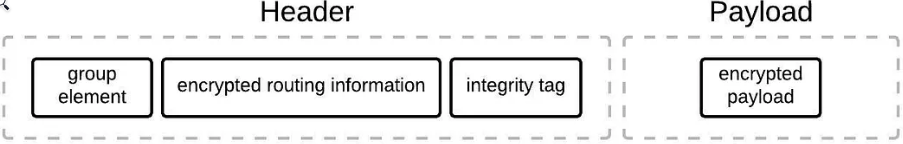
\includegraphics[width=0.9\linewidth]{Images/sphinx_structure.png}
    \caption{Structure of sphinx packet. \href{https://blog.nymtech.net/sphinx-tl-dr-the-data-packet-that-can-anonymize-bitcoin-and-the-internet-18d152c6e4dc}{[source]}}
    \label{fig:sphinx_structure}
\end{figure}

The \textit{encrypted routing information ($\beta$)} is constructed in layers, applied in reverse order along the path.
First, the final destination is encrypted, and an integrity tag ($\gamma_i$) is computed. 
The IP address of the last mixnode ($n_i$) is then prepended.
As shown by Figure \ref{fig:sphinx_header}, this process repeats iteratively: each new header is encrypted, an integrity tag ($\gamma_{i-1}$) is computed, and the IP address of the preceding mixnode ($n_{i-1}$) is prepended.
This layered encryption ensures that each mixnode can only decrypt its own layer, revealing the next forwarding address while preserving end-to-end confidentiality and protecting against tampering.

\begin{figure}[h]
    \centering
    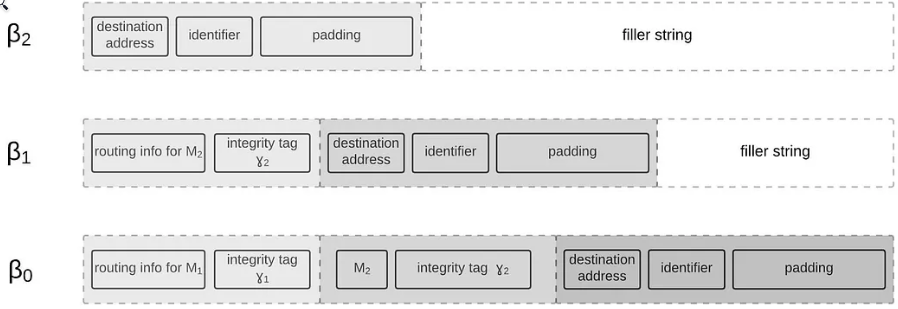
\includegraphics[width=\linewidth]{Images/sphinx_header.png}
    \caption{Sphinx encrypted routing information encapsulation. \href{https://blog.nymtech.net/sphinx-tl-dr-the-data-packet-that-can-anonymize-bitcoin-and-the-internet-18d152c6e4dc}{[source]}}
    \label{fig:sphinx_header}
\end{figure}

To encrypt the routing information, the Nym client\todo{previously "user" but JT prefers "Nym client"} first chooses a nonce $x$ and compute $\alpha = g^x$ as the \textit{cryptographic element} of the header.
Since each mixnode $i$ has a private key $x_i$ and a public key $y_i = g^{x_i}$, the user can create a shared secret $s_i$ with mixnode $i$ as followed: $s_i = y_i^x = (g^{x_i})^x$. 
Then the mixnode $i$ receiving the packet will get $\alpha$ allowing him to compute the shared secret as followed: $s_i = \alpha^{x_i} = (g^x)^{x_i}$.

Instead of sending a unique \textit{cryptographic element $\alpha$} at each node in the path, the sphinx format uses a single \textit{cryptographic element $\alpha$}, which is progressively modified at each node. 
Each mixnode updates the cryptographic element using its shared secret as follows:  
$$\alpha_{i+1} = \alpha_i^{\text{hash}(\alpha_i, s_i)}$$
Thus, the user iteratively computes the shared secrets in the path's order as: 
$$
\begin{aligned}
    \alpha_0 &= g^{x}, & s_0 &= y_{n_0}^{x}, & b_0 &= \text{hash}(\alpha_0, s_0) \\
    \alpha_1 &= g^{x b_0}, & s_1 &= y_{n_1}^{x b_0}, & b_1 &= \text{hash}(\alpha_1, s_1) \\
    &\vdots & &\vdots & &\vdots \\
    \alpha_i &= g^{x b_0 \cdots b_{i-1}}, & s_i &= y_{n_i}^{x b_0 \cdots b_{i-1}}, & b_i &= \text{hash}(\alpha_i, s_i)
\end{aligned}
$$
This formulation ensures that each mixnode can independently derive the necessary cryptographic elements without requiring the full path’s information, preserving privacy and unlinkability.  
\newline

The \textit{encrypted routing information ($\beta$)} is computed, as illustrated in Figure\todo{$\sim$\textbackslash ref\{\}} \ref{fig:sphinx_header}, by processing the path in reverse order. 
This involves XORing the routing information ($\beta_{i-1}$) from the previous layer (with the node's address and integrity tag) with a value derived from the shared secret $s_i$. 
Then prepending this new encrypted routing information ($\beta_i$) with an integrity tag ($\gamma_i$) and the previous mixnode address (remember we build it in reverse order).
We repeat the same process for each layer (i.e. each mixnode in the path).

\begin{figure}[H]
    \centering
    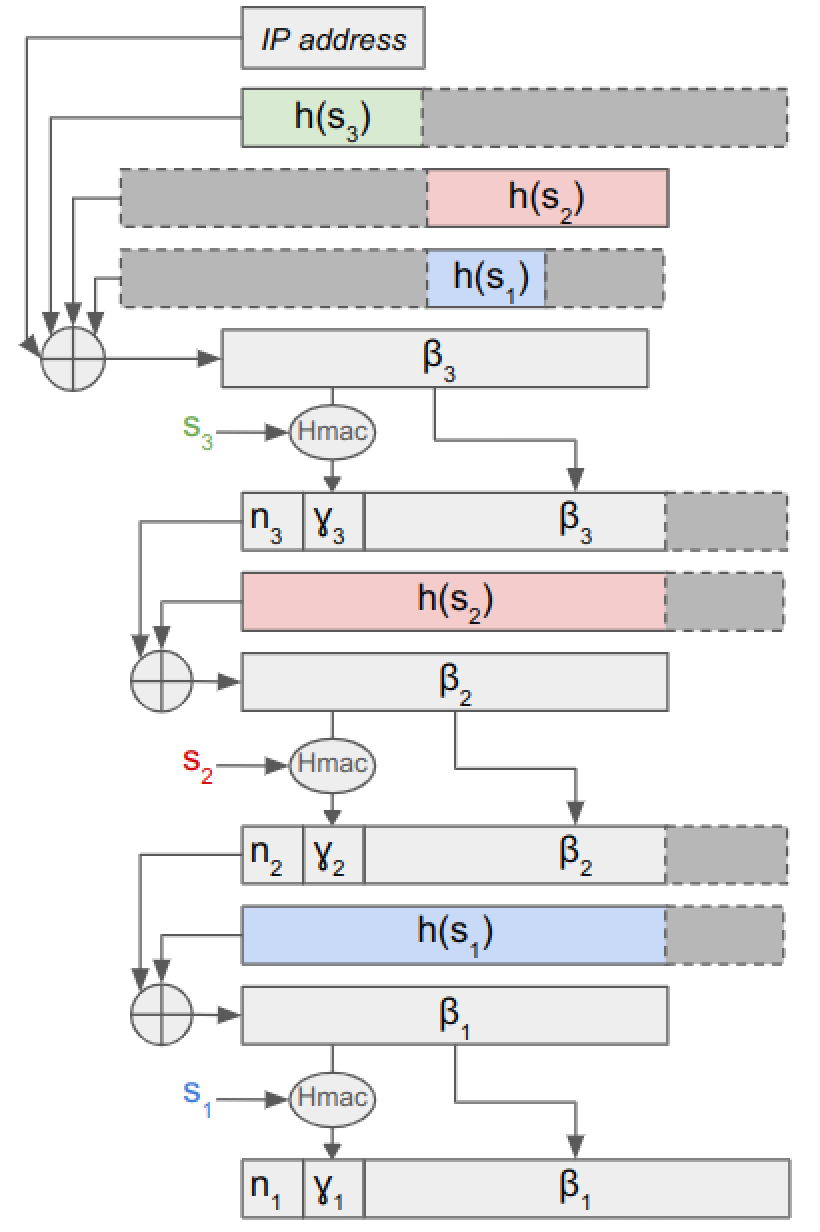
\includegraphics[width=0.5\linewidth]{Images/header_cipher.png}
    \caption{Construction of the Sphinx header (modified from \cite{sphinx}) [TO FIX: $h(s_1)$ at first XOR]}
    \label{fig:header_cipher}
\end{figure}
\todo[inline]{JT: Explain what the modifications are}
\todo[inline]{JT: Might help to put some (1) (2) (3) labels into the figure and refer to these labels in the text.}

% first round
The first round of XOR operations differs from the others because it requires combining parts of all shared secrets. 
Specifically, the destination address is XORed with the last node’s shared secret, truncated to match the address size.
Next, the result is concatenated with the XORed values of the ending parts of the shared secrets from the other nodes in the path. 
This ensures that when the entire header is XORed with the full shared secret, these appended values cancel out, allowing the header to be processed in reverse order by the mixnodes.
This design choice guarantees fixed-size headers, enabling fixed-size packets which is a crucial property in mixnets for maintaining unlinkability.

\todo[inline]{JT: Now maybe follow up with an example of the attack from the introduction?
We should also compare computational overheads from attack vs. the new protocol design.}

%%%%%%%%%%%%%%%%%%%%%%%%%%%%%%%%%%%%%%%%%%%%%%%%%%%%%%%%%%%%%%%%%%%%%%%%%%%%%%%%%%%%%%%%%%%%%%%%%%%%%%%%
%%%%%%%%%%%%%%%%%%%%%%%%%%%%%%%%%%%%%%%%% Our solution %%%%%%%%%%%%%%%%%%%%%%%%%%%%%%%%%%%%%%%%%%%%%%%%%
%%%%%%%%%%%%%%%%%%%%%%%%%%%%%%%%%%%%%%%%%%%%%%%%%%%%%%%%%%%%%%%%%%%%%%%%%%%%%%%%%%%%%%%%%%%%%%%%%%%%%%%%

\newpage
\section{Our Solution - Multi-Party Computation (MPC)}\label{sec:scheme}
\todo[inline, color=blue!30]
{
    [NOTE] - To do or improve
        \newline- Carefully select variable's notation, e.g. h, h(), H() and hash();
        \newline\hspace*{1cm} - Don't like $\alpha$ notation since it should be capital letter (point)
        \newline\hspace*{1cm} - Should use $\Gamma$ instead of $\gamma$ notation (point)
        \newline\hspace*{1cm} - And what about $\beta$, $b$, $x$, ...
        \newline- Do or improve schemas;
        \newline- Clarify that we work with a path of length 3 (could be generalized)
}

The first approach to ensure trust in the Sphinx header is to prevent user manipulation by decentralizing the header construction to Trusted Third Parties (TTP) through the use of Multi-Party Computaftion (MPC).
\newline

We consider TTPs as \textit{honest-but-curious}.
This means that they follow the protocol correctly but may attempt to infer additional information from the data they process.
Our design ensures that TTPs cannot infer any information about the shared secrets $ s_i $ or the involved mixnodes, even when TTPs collude (except one).
\todo{JT: In the Nym ecosystem, who are the TTPs, who operates them, what exactly are they trusted for?}

\subsection{Development Path / Thinking path}

Before introducing our decentralized schema, we briefly outline the key decisions that shaped our implementation.
\newline

\noindent We considered three main approaches to decentralize the Sphinx header computation:
\begin{enumerate}
    \item \textbf{Distributed:} Each TTP computes a distinct layer (sequential approach);
    \item \textbf{Partially decentralized:} All TTPs compute a layer based on partial information, aggregate their results to compute the integrity hash, redistribute the outcome, and repeat the process with the next layer;
    \item \textbf{Fully decentralized:} All TTPs compute the full Sphinx header using partial information, and their results are aggregated at the end.
\end{enumerate}

The first approach compromises privacy, as each TTP learns two consecutive nodes in the path and one of the associated shared secrets, raising serious security concerns.
The second approach increases communication overhead and allows the aggregating TTP to observe the intermediate Sphinx header at specific stages, which could enable packet tracking if the aggregator colludes.
Finally, the third approach was selected for its stronger privacy guarantees, despite its added complexity.
\newline

% hash -> Homomorphic encryption
The main challenge in the fully decentralized setting lies in the integrity tag which relies on a hash function. 
Although a homomorphic hash would be ideal to support decentralized hash, such construction remains poorly studied and potentially weaken its security due to the homomorphic additive or multiplicative nature (easier for collisions).
As a practical workaround, we substitute the hash with a one-way homomorphic encryption scheme (only encryption, not decryption). 
More specifically, a homomorphic encryption with mutually commutative operators (like RSA and ElGamal but not Paillier) due to the nested structure of the integrity tag, which contains previous tags.
\todo[color=blue!30]{Should I develop why ?}

%%% Size -> ECC -> 1 Point per element -> cut in chunks
To improve efficiency, we switch from RSA-like primitives to elliptic curve cryptography (ECC), which offers more compact representations while keeping these homomorphic properties.
By abstracting away encryption layers, the final header is structured as follows: 
\[
[\text{node 1, integrity 1, node 2, integrity 2, node 3, integrity 3, destination}]
\]
\todo[color=blue!30]{adding a figure to illustrate ?}
Since deriving all these information from just one or two EC points seems impractical, we represent each piece of information by an EC point.
To achieve this, we split the encoded string into chunks as represented by Figure \ref{fig:chunked_schema}, each corresponding to a single EC point.

\begin{figure}[H]
    \centering
    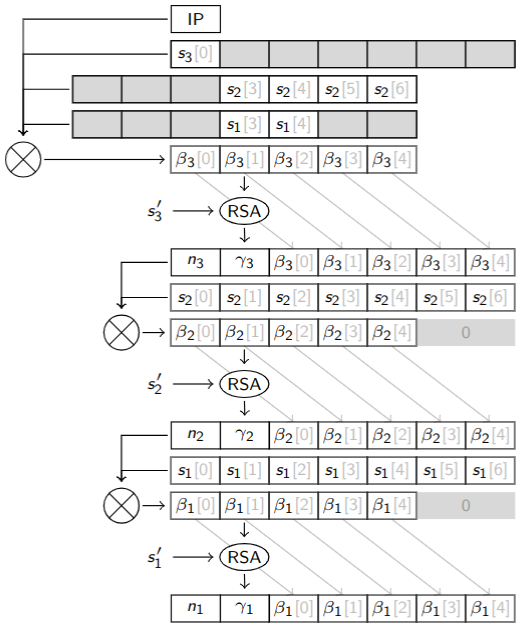
\includegraphics[width=0.6\linewidth]{Images/chunked_structure.png}
    \caption{Chunked representation of the schema}
    \label{fig:chunked_schema}
\end{figure}

\todo[color=blue!20]{Nice guidelines ref: RFC9380 (Hashing to Elliptic Curves)}
One remaining challenge when encoding information into elliptic curve (EC) points is the decoding process.  
Some type of data such as IP addresses (destination or mixnodes) requires both an encoding method that maps an integer to a point and a corresponding decoding method that retrieves the integer from the point.
In this article, we refer to these two processes respectively as \textit{integer-to-point} noted $H()$, and \textit{point-to-integer} noted $h()$.
\newline

A classical approach to achieve such a mapping involves the x-coordinate of the point.
The point-to-integer function simply returns the x-coordinate of the point.
The integer-to-point function computes the y-coordinate where x is the integer.
However, a randomly chosen x-coordinate will lie on the curve only about 50\% of the time.  
A simple workaround is to increment the x-coordinate until a valid point is found.  
Yet, this technique introduces a problem in our context since the x-coordinates correspond to IP addresses. 
Nearby IPs could map to the same point, potentially leading to collisions that compromise correctness of the mixnet.
This risk could be mitigated by padding the IP with a random fixed-length binary string.
\newline

From our knowledge, a second alternative exists: the Elligator 2 algorithm.  
Elligator provides a method to map any integer to a pseudo-random point on a Montgomery curve in a uniform and reversible way.  
More precisely, the reverse mapping (point-to-integer) requires that the point satisfies specific mathematical conditions, which occur with roughly 50\% probability for a random point.  
Again, a simple workaround is to increment the point by adding the curve's generator until the point fulfills these conditions.

Note that all points derived from integers using Elligator are guaranteed to be reversible.  
Thus, a point representing an IP address (which originally comes from an integers) can always be correctly decoded.  
Only random points used as shared secrets may require few extra point additions to meet these conditions which represents a negligible computational overhead.
\newline

To summarize, we need a mapping that is as bijective as possible but we face a trade-off between two imperfect scenarios:
\begin{itemize}
    \item A complete and easily reversible point-to-integer mapping (i.e. using x-coordinates), but only partial coverage for integer-to-point.
    \item A complete integer-to-point mapping (i.e. using Elligator), but only partial coverage for point-to-integer.
\end{itemize}

Elligator seems a better solution since it guarantees stronger security/privacy by providing a more uniformly distributed output.
Moreover the complete integer-to-point is more important (to prevent IP collision) and we can deal with partial point-to-integer mapping in our use case.

\newpage
\todo[inline, color=blue!30]{
    It feels a bit heavy with too much details and remarks. 
    The whole previous page could be reduced to this shorter alternative.
    Which one is better ?
    \newline

    [Alternative shorter version]: \newline
    One remaining challenge lies in encoding and decoding information to and from elliptic curve points. 
    Specifically, we require a pseudo-random mapping between integers field and curve points group.
    
    Traditional methods achieve this by directly mapping integers to the x-coordinates of points on the curve. 
    However, this approach could leaks information by introducing bias since nearby integers result in nearby points.
    
    To address this, we adopt Elligator, which offers stronger privacy guarantees. 
    Unlike the traditional approach, Elligator produces a uniformly distributed output which is computationally indistinguishable from truly random curve points. 
    This uniformity is critical in our context, where preserving anonymity and avoiding linkability are core goals.
}

\subsection{Protocol description}

The overall decentralized scheme is illustrated in Figure~\ref{fig:overall_schema}.  
The client first computes a sequence of shared secrets and then splits these secrets, along with the IP addresses of the mixnodes in the path and the final destination, into $m$ shares.  
Each set of shares is sent to a different TTP, along with the necessary cryptographic element ($\alpha$).  
Each TTP independently computes a \textit{partial} Sphinx header using the received shares.  
The client then aggregates these partial headers to reconstruct the final header, ready for transmission through the mixnet.

\begin{figure}[H]
    \centering
    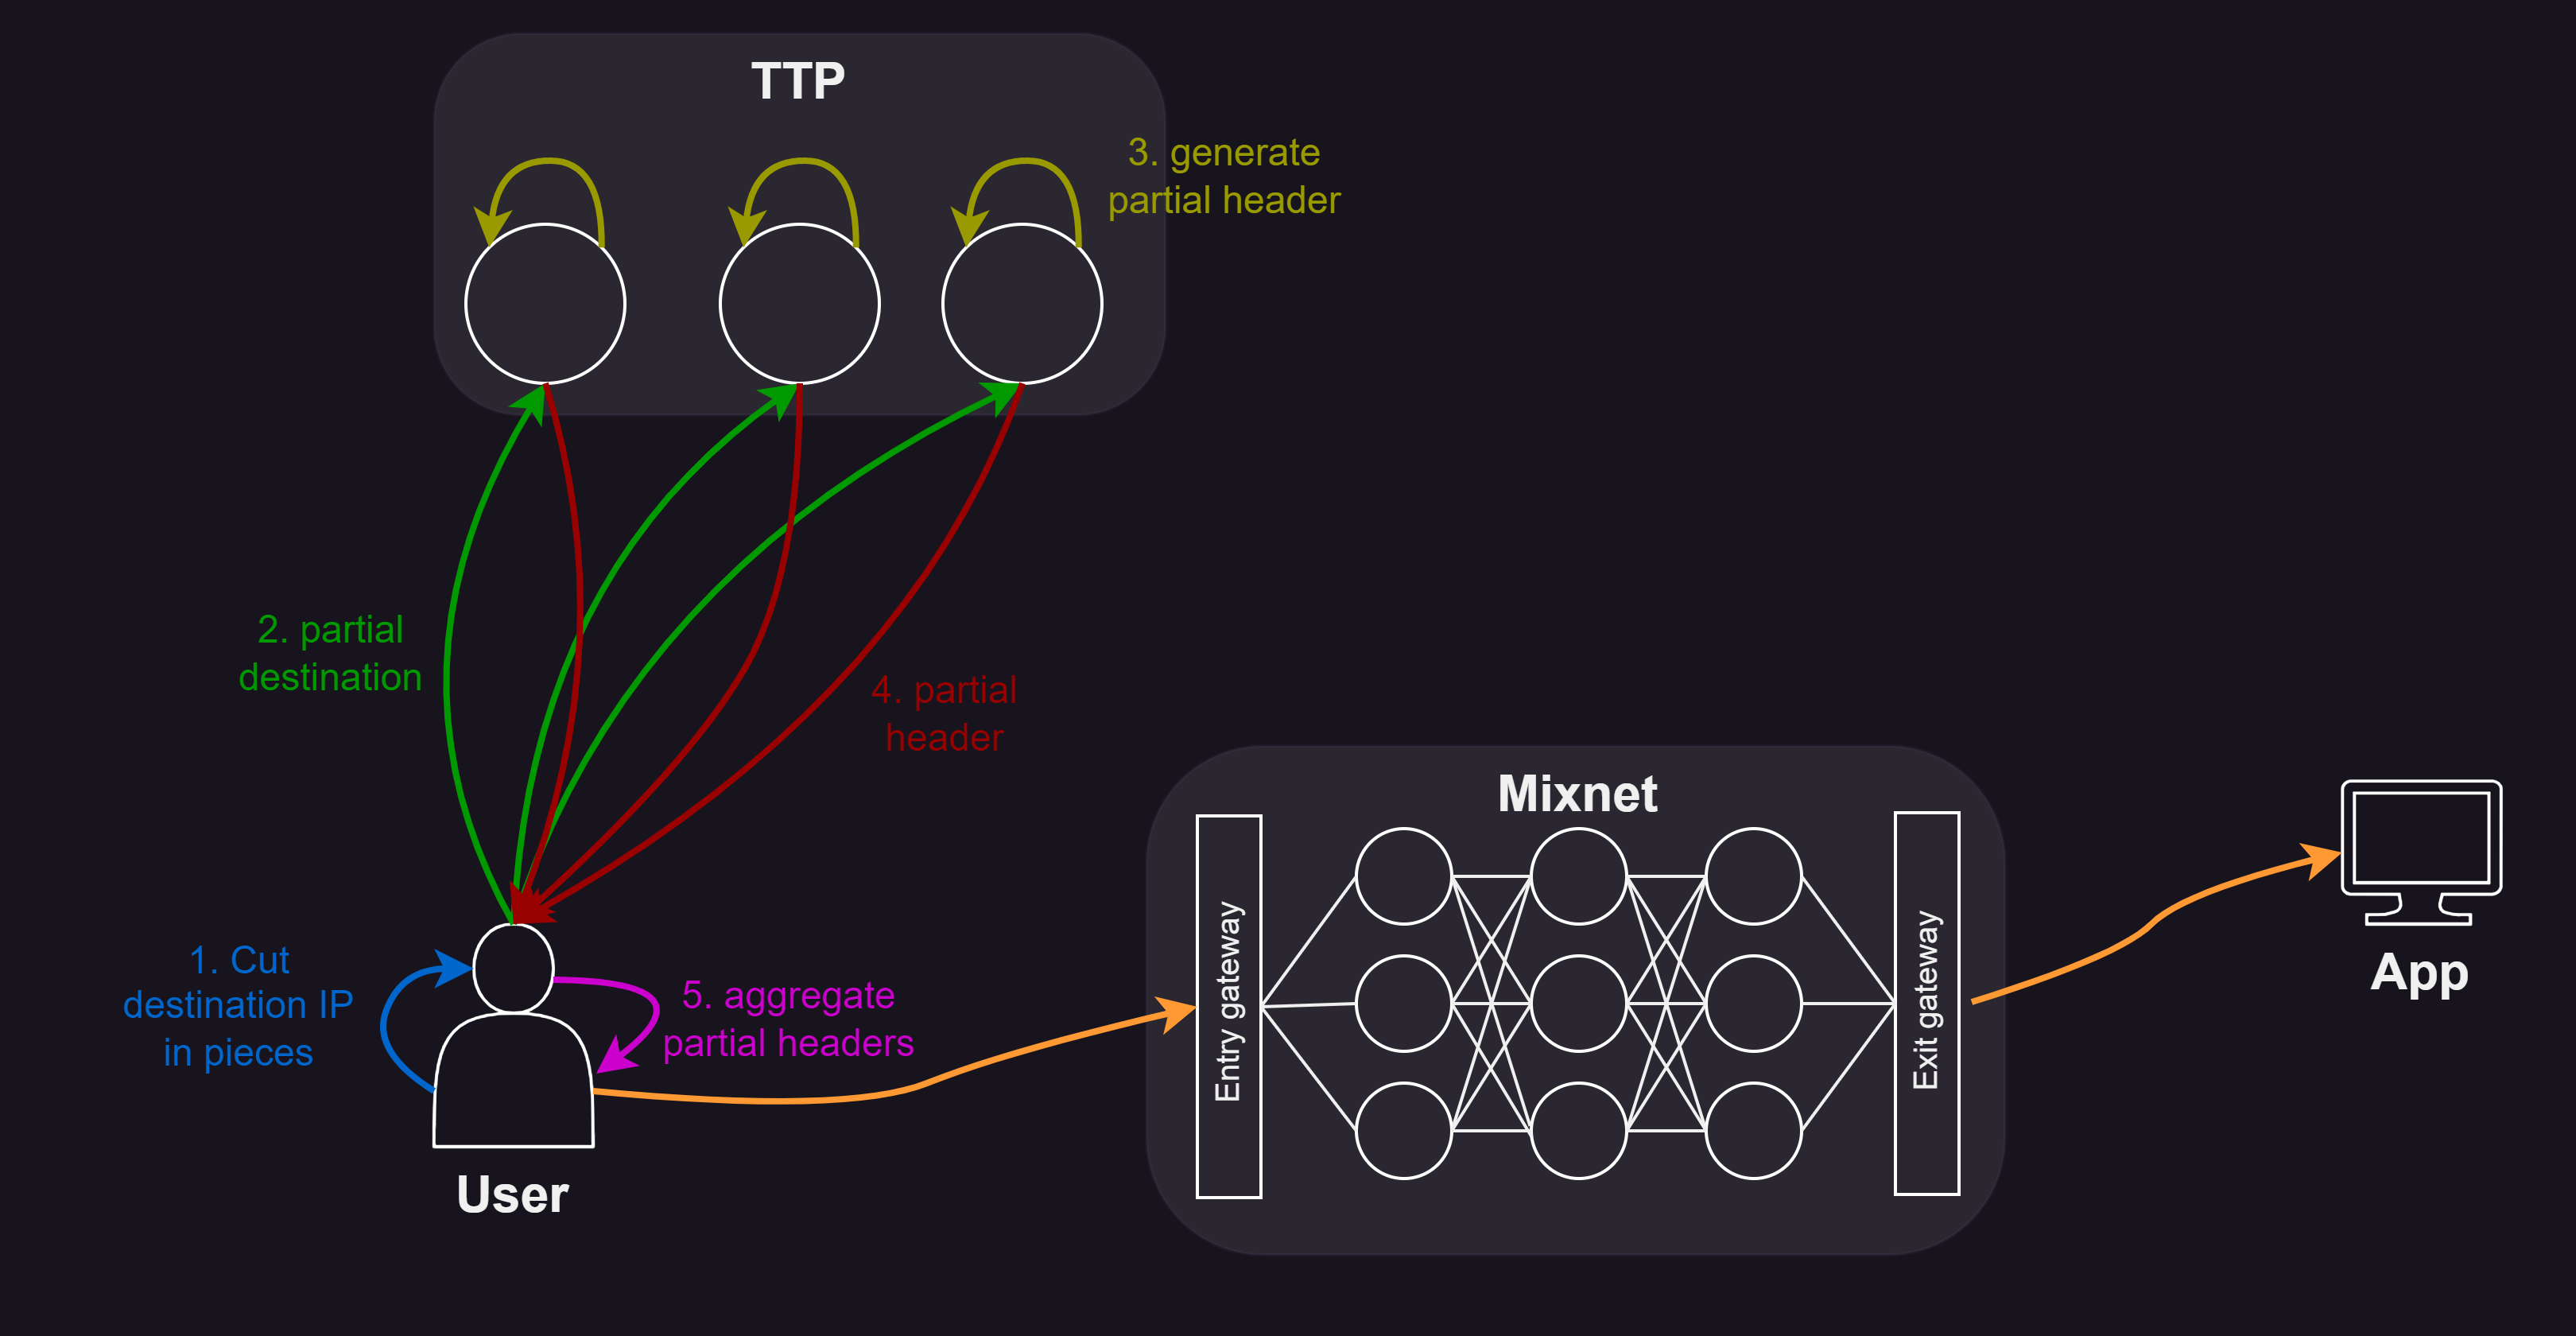
\includegraphics[width=1\linewidth]{Images/sphinx_ttp.png}
    \caption{Overview of the decentralized scheme}
    \label{fig:overall_schema}
\end{figure}

\noindent In summary, the protocol is divided into four main steps:
\begin{itemize}
    \item \textbf{Setup}: fixes random points as \textit{generators} (once but should be refreshed);
    \item \textbf{Client}: \textit{splits and shares} the necessary information to TTPs;
    \item \textbf{TTP}: \textit{encrypts} the routing information into a partial header;
    \item \textbf{Mixnode}: \textit{decrypts} and forwards the header.
\end{itemize}


\subsubsection{Setup}

In our protocol, routing information is divided into seven chunks (see Figure \ref{fig:chunked_schema}), each one encoded into an elliptic curve point. 
These points will later be encrypted by adding a masking point of the form $ P = s G $, where $ s $ is a shared secret and $ G $ is the base generator of the curve.
However, using the same masking point $ P $ for all the seven chunks compromises the \textit{unlinkability} property
(see security note in the TTP step \ref{note:security_why_indep_generators}).

To mitigate this, we use a set of seven \textit{independent} generators $ G_i $, one for each chunk. 
By \textit{independent}, we mean that the scalar relationship between any two generators is unknown. 
Therefore no one knows the scalars $ x_i \in \mathbb{Z}_N $ such that $ G_i = x_i G $.

In principle, this setup phase can be executed only once. 
However, to preserve unlinkability, the set of generators should be refreshed periodically. 
Every entity (clients, mixnodes, and TTPs) must run the setup phase to ensure they use the same set of generators.

To achieve synchronized and deterministic generator values across the system, we derive them from a common seed. 
This seed is computed as the hash of the current timestamp, truncated to the chosen refresh interval. 
To produce distinct seeds for each generator we rehash the seed, or simply increment it since Elligator already provides a uniform (i.e. pseudo-random) integers to points mapping.
\todo[color=blue!30]{In the current implementation, instead of incrementing the seed, we rehash it for each i. However, since Elligator produces uniformly distributed outputs, incrementing may be equally secure and more efficient.}

A subtlety with Elligator is that it can map integers to points outside of the base generator's subgroup.
Thus, an extra step is required to \textit{clear the cofactor} by multiplying the resulting point by the cofactor $ h $ (for Curve25519, $ h = 8 $).

\noindent The final formula for generating the $ i^{th} $ chunk’s generator is:
$$
G_i = h \cdot H(\text{hash}(\text{timestamp}) + i), \quad \text{for } i = 1, \dots, 7
$$


\subsubsection{Client}
% 1) Define a destination
% 2) Select a random path
% 3) Select a random salt $x$ (nonce) 
% 4) Generate a chain of shared secret for the path's mixnode
% 5) Transform IP addresses (path's mixnodes and destination) into Point with Elligator and the split those point into shares.
% 6) Split the shared secrets (int) into shares.
% 7) Send sets of shares (mixnodes IPs, destination IP, shared secrets) to different TTP.
% 8) TTP will compute from those shares a partial header and send it to the client. Afterwards, the client aggregate these partial headers.
  
To send a message to a specific destination, the client first randomly chooses a path through the mixnet and generates a nonce.
Using this nonce and the public keys of each mixnode along the path, the client derives a chain of shared secret integers $ (s_1, s_2, s_3) $ as follows:
\todo[inline,color=blue!30]
{
    Does it seems strange to transform the shared secret point into integer ?
    Should I explain why we need integer form ? 
    It might be a bit heavy and add too much details...
}
$$
\begin{aligned}
    \alpha_i    &= x_i \, G \\
    S_i         &= x_i \, \text{PK}_i \\
    s_i         &= h(S_i) \\
    b_i         &= \text{hash} ( {\alpha_i}_y \ \| \ {S_i}_y ) \\
    x_{i+1}     &= x_i \, b_i \quad (\text{mod}\ N)
\end{aligned}
$$
\todo[color=blue!30]{Order of equation lines ? and names of variables (espacially $x_i$ and $b_i$) ?}
where $ x_1 $ is the client's nonce, $ \text{PK}_i $ is the public key of the $ i^{th} $ mixnode in the path, 
$ N $ is the prime order of the elliptic curve group, $ \| $ is  the concatenation operator and subscript $ y $ refers to the $ y $-coordinate of the point.
The scalar $ b_i $ acts as a pseudo-randomizer to update the secret $ x_i $ for the next hop, 
ensuring that each cryptographic element $ \alpha_i $ remains unlinkable across mixnodes.

The IP addresses of the mixnodes and the destination are padded with random bits
then mapped to elliptic curve points using Elligator, allowing later recovery of these addresses.
\todo[color=red!40]{Test code: to verify if the padding is still necessary or optionnal and if limited (max size N)}
Both the resulting IP points and the shared secrets are split into shares and distributed to $ m $ different TTPs. 
\todo[inline, color=blue!30]{Should I mention how to split point (or integer) into $ m $ shares ? 
It is just taking $ m - 1 $ random points (or integers), sum them and compute the difference with the original point (or integer).}


Each TTP then independently computes a partial header from the received shares and returns it to the client. 
The client aggregates these partial headers by performing chunkwise point additions to reconstruct the complete encrypted header.
Finally, the client sends the header along with $ \alpha_1 $ to the first mixnode from the path. 
\todo[color=blue!30]{Do we need to remind that the user need to encrypt his message using these shared secrets (as in original article) or is uninteresting/obvious enough ?}

\subsubsection{TTP}
% 1) Receive partial destination, path's nodes and partial shared secret
% 2) First
% 3) For each layer
Each TTP receives from the client:
\begin{itemize}
    \item a share of the destination address (as an elliptic curve point),
    \item a share of each mixnode address in the path (as elliptic curve points),
    \item a share of each shared secrets (as integers).
\end{itemize}

The TTP constructs a partial encrypted header by layering routing information in reverse path order, starting from the last mixnode.

At each layer, two new chunks are introduced: the next mixnode’s address (as an EC point) and an integrity tag.  
To preserve a fixed-length header while allowing mixnodes to reverse the operation (as in the original design), four additional \emph{filler chunks} are appended.  
These filler chunks are carefully computed such that at each layer, after applying the corresponding masking points ($s_i \ G_j$), the last two chunks cancel out and become identity point (i.e. point at infinity).  
This mechanism allows these two chunks to be safely truncated at each layer, ensuring a consistent header size while preserving reversibility for mixnodes.

To initialize the header, the TTP encrypts the destination point using the shared secret of the last mixnode and append the required filler chunks. 
Let $ \Delta $ be the partial destination point, $ s_i $ the shared secret corresponding to the $ i^\text{th} $ mixnode in the path, and $ G_j $ the $ j^\text{th} $ chunk's generator. 
The chunks for the last layer (layer 3, assuming a 3-hop path) are computed as follows:

\[
\begin{aligned}
    {\beta_3}_1 &= \Delta       + s_3 \ G_1 \\
    {\beta_3}_2 &= - (s_2 \ G_4 + s_1 \ G_6) \\
    {\beta_3}_3 &= - (s_2 \ G_5 + s_1 \ G_7) \\
    {\beta_3}_4 &= - s_2 \ G_6 \\
    {\beta_3}_5 &= - s_2 \ G_7 \\
\end{aligned}
\]
The integrity tag for this layer is computed as:
\[
\gamma_3 = s_3 \ G + \sum_{j=1}^{5} {\beta_3}_j
\]
Subsequent layers (for $ i = 2 $ and $ i = 1 $) are computed as:
\[
\begin{aligned}
    {\beta_i}_1 &= N_{i+1} + s_i \ G_1\\
    {\beta_i}_2 &= \gamma_{i+1} + s_i \ G_2 \\
    {\beta_i}_3 &= {\beta_{i+1}}_1 + s_i \ G_3 \\
    {\beta_i}_4 &= {\beta_{i+1}}_2 + s_i \ G_4 \\
    {\beta_i}_5 &= {\beta_{i+1}}_3 + s_i \ G_5 \\
\end{aligned}
\]
with the corresponding integrity tag:
\[
\gamma_i = s_i \ G + \sum_{j=1}^{5} {\beta_i}_j
\]
Here, $ N_{i+1} $ represents the elliptic curve point corresponding to the $ (i+1)^\text{th} $ mixnode in the path.

When the first layer is finally computed, it is appended with the first mixnode’s point $ N_1 $ and the integrity tag $ \gamma_1 $.
Finally, the TTP returns the constructed partial header to the client.

\paragraph{\textbf{Security Note.}}\label{note:security_why_indep_generators}
To preserve unlinkability, it is essential that the generators $ (G_1, \dots, G_7) $ are \textit{independent}, meaning that their scalar relationships are unknown and cannot be derived.
If the same generator $ G' $ were used across chunks (or their scalar relationships known), an adversary could compute the chunk-wise difference between consecutive layers: $ {\beta_i}_j - {\beta_{i+1}}_j = s_i \ G' $.
Since the shared secret $ s_i $ remains consistent within a layer, the resulting differences would reveal a predictable pattern (uniform or preserved scalar relationships).
This consistency could allow an adversary to correlate incoming and outgoing packets at a mixnode, thereby breaking the unlinkability property.
Using independent generators for each chunk prevents such correlations and is therefore critical to the protocol's security.  
  

\subsubsection{Mixnode}
% 1) Extract information from the header
% 2) Recompute shared secret
% 3) Integrity check
% 4) Update encrypted information (β)
% 5) Update cryptographic element (α)


When a packet arrives at a mixnode, it begins by extracting the relevant header fields, namely the cryptographic element $ \alpha $ and the integrity tag $ \gamma $.  
The mixnode then recomputes the shared secret point $ S $ using its private key $ \text{sk} $ and the cryptographic element $ \alpha $:  
\[
S = \text{sk} \ \alpha
\]
This point is subsequently mapped to a shared secret integer $ s $ using Elligator.
This shared secret integer is then used to verify the integrity tag: 
\[
\gamma \overset{\text{?}}{=} s \ G + \sum_{j=1}^{5} \beta_j
\]
The integrity tag is constructed as the sum of the chunks, offset by a secret point derived from the shared secret integer. 
This ensures that only the client and intended mixnode can create, modify, or verify it.

\noindent If the integrity check passes, the mixnode pads the header by appending two \textit{identity} chunks (i.e. point at infinity) and then updates it as:
\[
\beta'_j = \beta_j - s \ G_j \qquad \forall j = 1, \dots, 7
\]

The first chunk ($ \beta'_1 $), encodes the next mixnode’s IP address. 
This point is mapped back to an integer using Elligator and the random padding is removed by keeping the last 128 bits (i.e. size of IP address).

\noindent The second chunk ($ \beta'_2 $) is the new integrity tag ($ \gamma' $) for the remaining five chunks that form the new encrypted routing information ($ \beta' $).

To maintain unlinkability, the cryptographic element $ \alpha $ must be updated for the next hop. 
As in the client's step, it is computed using the $y$-coordinates of both $ \alpha $ and $ S $:
\[
\alpha' = \text{hash}(\alpha_y \ \| \ S_y) \ \alpha
\]
Finally, the mixnode forwards the updated header $ (\alpha', \gamma', \beta') $ to the next node.
